\documentclass[12pt]{article}
\usepackage[english]{babel}
\usepackage[margin=0.80in]{geometry}
\usepackage{amsmath}
\usepackage{amssymb}
\usepackage{algorithm}
\usepackage[noend]{algpseudocode}
\usepackage[utf8]{inputenc}
\usepackage{graphicx}
\usepackage{listings}
\usepackage{color}
\usepackage{hyperref}
\usepackage{cite}
%\usepackage{textcomp,uiosloforside}
\numberwithin{figure}{section}
\numberwithin{table}{section}

\definecolor{mygreen}{rgb}{0,0.6,0}
\definecolor{mymauve}{rgb}{0.58,0,0.82}
\definecolor{mygray}{rgb}{0.97,0.97,0.97}
  
\lstset{
  language=C++,
  basicstyle=\footnotesize,
  commentstyle=\color{mygreen},
  keywordstyle=\color{blue},
  stringstyle=\color{mymauve},
  tabsize=4
}

\begin{document}
\begin{titlepage}
\title{Project 3 - FYS4150}
\author{Oda Langrekken, Trude Hjelmeland and Jostein Brændshøi}
\date{
    Department of Physics\\%
    University of Oslo\\[2ex]%
    \today
}
\clearpage
\maketitle
\thispagestyle{empty}

\begin{abstract}
\noindent We use the Euler and Velocity Verlet algorithms to simulate the motion of the Earth around the Sun, and later we use the latter method to model the entire Solar System. We discover that the Verlet method is by far superior to the Euler method regarding precision, conservation of energy and angular momentum, and that it nearly matches the Euler method in terms of time efficiency. Experimenting with our model, we also discover that changing the properties of the planets or the distance-dependency of the gravitational force, has dramatic consequences for our Solar System.
\end{abstract}
\vspace{2.00cm}

\noindent The address \url{https://github.com/jostbr/FYS4150-Projects/tree/master/Project3} on Git-Hub is associated with this project. Here one can find all code used in the project. This includes C++ source files containing the core of the project, but also a Python plotting script for result visualization. There are also available benchmark results from running the code as well as \LaTeX \ source for this PDF. In addition some animations (generated with the python script) are uploaded to YouTube are associated with this project and the specifics links are provided below in the report when relevant.

\end{titlepage}
\pagebreak

\tableofcontents
\pagebreak

% ======== Indicate new section
% -------- Indicate new subsection

% ========================================================================================
% ========================================================================================
\section{Introduction}

\noindent The motion of any classical object of constant mass experiencing some force, can be described by Newton's second law
\begin{equation}
   F=ma
\end{equation}
All high school student taking a course in physics, will have solved this equation for a number of simple systems with constant acceleration (the motion of an object moving on a frictionless plane is perhaps the most well-known example). If the acceleration is not constant, but rather some function of position, the situation becomes more complex as one will have to solve a second order differential equation to calculate the motion. Sometimes the equation can still be solved analytically, but more than often this is not possible. Luckily we have tools to find approximate solutions to these equations, namely numerical algorithms. \\

\noindent The aim of this project is to simulate the evolution of our Solar System by solving coupled ordinary differential equations using numerical methods in an object oriented manner. By first utilizing the forward Euler method we will see that the velocity Verlet is a more fitting algorithm to employ as the latter conserves the energy of the system, and thus provides a more stable solution. \\

\noindent First we will discuss the theory used in this project, most notably Newton's Second Law for many body systems.  We then move on to explain how the equations can be discretized and solved using the Euler and Verlet method. Next we introduce some of the tests we have performed on our model to test the precision. We then present our results and how they can be interpreted. Finally we offer some reflections and personal insight gained from working with this project.\\


%====================================================================================
%====================================================================================
\section{Theory} \label{sec:theory}
 
\subsection{Newton's Second Law }
\noindent  Newton's second law  states that the force $\mathbf{F}$ acting on a body is equal to the mass, $m$, multiplied by the acceleration, $\mathbf{a}$, of that body \cite{newton-principia}; 

\begin{equation}
	\label{N2L}
      \mathbf{F} = m\mathbf{a} = m \frac{d^2 \mathbf{r}}{dt^2}
\end{equation}

\noindent This equation is valid for all systems where the masses are constant, which we will assume is the case in our project. This is, however, a truth with some modifications (i.e. the Sun is reducing it's mass by a fraction of $10^{-13}$ every year \cite{solar}). \\

\noindent The above equation \eqref{N2L} is a second order ordinary differential equation that can be rewritten as two coupled first order ordinary differential equations \cite{Comp} by;



\begin{equation}
		\label{dr/dt}
         \frac{d\mathbf{r}}{dt}=\mathbf{v}(\mathbf{r},t)
\end{equation}

\begin{equation}
		\label{dv/dt}
         \frac{d \mathbf{v}}{dt} = \mathbf{a}(\mathbf{r}, t) 
\end{equation}



%Could include section on law of conservation of energy.  
\noindent To solve a set of coupled ordinary differential equations we need to know the initial values at some initial time $t_0$ for both position and velocity, namely $\mathbf{r}(t_0)$ and $\mathbf{v}(t_0)$ which we will discuss more in section \ref{sec:methods}. \\







%------------------------------------------------------------------------------
\subsection{Earth-Sun System}
\label{Earth-Sun}

\noindent In the first part of our project we will simplify our system by limiting ourselves to only one planet orbiting a star, namely the Earth orbiting the Sun.\\
 
\noindent The motion of the Earth is governed by the universal law of gravitation, formulated by Sir Isaac Newton \cite{newton-principia}. The law states states that two point masses are attracted to each other by a force that is directly proportional to the masses of the bodies and inversely proportional to the distance between their two mass centers, $r$, squared; 

\begin{equation}
		\label{Gforce}
        \mathbf{F} = G \frac{m_1 m_2}{r^2}\hat{\mathbf{r}}
\end{equation}
\noindent where $\hat{\mathbf{r}}$ is the unit vector pointing from the body experiencing the force to the object exerting the force.  Thus the gravitational attraction is a central force, meaning that the force is directed along a straight line passing through the centers of the interacting bodies \cite{VGS-FYS}.  \\
\noindent The gravitational constant, G, was found through experiments to be $6.67\times 10^{-11} \frac{m^3}{kg\times s^2}$.\\
\noindent Because the size of the planets is very small compared to the distance between them, we will approximate the planets and the Sun as point particles. \\

\noindent Assuming circular orbits, the acceleration of the Earth is described by the centripetal acceleration. Inserting the centripetal acceleration in Newton's Second Law \eqref{N2L}, using gravitation \eqref{Gforce} as the force and solving for the Earth's acceleration in this simplified two body Solar System yields;

\begin{equation}
	a_E = \frac{v_E^2}{r} = \frac{F}{M_E} =  \frac{G M_S}{r^2}
\end{equation}

\noindent where $M_E$ and $M_S$ is the mass of the Earth and the Sun respectively.\\
This leads to the relationship $v^2 r = G M_S$.\\

\noindent To avoid working with very large numbers (which easily leads to loss of numerical precision) we scale our equations. Lengths will be measured in units of astronomical units (AU) where  1 AU is the mean distance between the Earth and the Sun. For the velocities we choose to work in units of AU/year. \\

\noindent Assuming circular orbits, we have $r=1$ AU and $v=2\pi $ AU/year as $2\pi $ AU is the circumference of a full orbit. Plugging this back into $v^2 r = G M_S$ we see that $G M_S = 4 \pi^2\frac{(\textnormal{AU})^3}{(\textnormal{year})^2}$ for our simplified system. \\

\noindent To further simplify our system, we decompose the acceleration of the Earth. For the x-direction , this leads to the expression

\begin{equation}
	\label{simple ax}
     a_x=a\cos\theta = - \frac{4\pi^2\cos\theta}{r^2} = - \frac{4 \pi^2 x_E}{r_{ES}^3}
\end{equation}

\noindent where we have used that the x-component of the position of the Earth, $x_E$, can be expressed as $x_e=r_{ES}\cos\theta$ where $r_{ES}$ is the distance between the Earth and the Sun. Similar expressions can be found for the y- and z-directions, where $x_e$ will be replaced by $y_e$ and $z_e$ respecitvely.  \\



%-----------------------------------------------------------------------------------
%-----------------------------------------------------------------------------------
\subsection{The Three Body System}
\noindent The Solar System does not, however, consist only of the Earth and the Sun. Proceeding with our project we want to include more planets in our solar system, and we will start by expanding our system to include the planet Jupiter. If we continue on with our simplified system described in the section above (section \ref{Earth-Sun}), we can include the gravitational force on the Earth from Jupiter by simply expanding the expression in equation \eqref{simple ax} with a additional term, namely;

\begin{equation}
		\label{three ax}
		a_x = - \frac{4 \pi^2 x_E}{r_{ES}^3} - \frac{4 \pi^2 \frac{M_J}{M_S} (x_E-x_J)}{r_{EJ}^3}
\end{equation}

\noindent  where we have used $$GM_J=G\frac{M_S}{M_J}=4\pi^2\frac{M_J}{M_S}$$This needs to be calculated for all the spatial directions and we need to add a similar set of equations for Jupiter's acceleration. \\ 


%-----------------------------------------------------------------------------------
%-----------------------------------------------------------------------------------
\subsection{The Solar System}
%Here we find the center of mass  
\noindent To finalize our project we want to include all $N=9$ planets of the Solar System in the simulation. We do this by expanding the calculation of the accelerations as shown in equation \eqref{three ax} to include all planets and thereby all pair of planets.  To simultaneously make the calculation as close to reality as possible, we want to include the motion of the Sun. This would imply that the sun is no longer some special case fixed at the origin, but rather treated as a planet just like the other planets. To be even more general we may think of this purely as an $N$-body system. In an $N$-body system we have $N$ bodies (in our case planets) all interacting with each other with some force (in the following discussion we will use gravity, however the approach stated below applies to any force that is inversely porportional to $r^2$, e.g. Coulomb force etc.). In particular the gravitational vector force between body $i$ and body $j$ can be, following \eqref{Gforce}, expressed as
%I think we should keep it as it is, but if you want to move it.. No problem. -Trude

\begin{equation}
	\mathbf{F}_i=G\frac{m_im_k}{|\mathbf{r}_i-\mathbf{r}_k|^3}(\mathbf{r}_i-\mathbf{r}_k) \label{eq:force_ik}
\end{equation}
and Newtons second \eqref{N2L} law for body $i$ reads
\begin{equation}
	\mathbf{F}_i=m_i\frac{d^2\mathbf{r}_i}{dt^2} \label{eq:N2L_vec}
\end{equation}
and combining \eqref{eq:force_ik} with \eqref{eq:N2L_vec} by summing up all the forces acting on body $i$ gives the second order vector differential equation
\begin{equation}
	m_i\frac{d^2\mathbf{r}_i}{dt^2}=\sum_{k=1}^NG\frac{m_im_k}{|\mathbf{r}_i-\mathbf{r}_k|^3}(\mathbf{r}_i-\mathbf{r}_k) \label{eq:N2L_nbody}
\end{equation}
for body $i$. We have one such equation for each of the $N$ bodies. Also the vector equation implies one equation for each direction, i.e. three equations per body, resulting in a total of $3N$ second order differential equations. \\

\noindent Another interesting aspect with such an $N$-body system is its mass center. By using a weighted average of the position vectors of each planet with each planet position weighted by its respective mass we can write
\begin{equation}
		\mathbf{r}_M=\frac{1}{M}\sum_{i=1}^Nm_i\mathbf{r}_i\label{center of mass}        
\end{equation}
where
\begin{equation}
	M=\sum_{i=1}^Nm_i
\end{equation}
is the total mass of the system and $\mathbf{r}_i$ is the position vector of planet $i$. We will utilize this in the result section to examine how good of an approximation it is to treat the Sun as fixed in the origin vs fully accounting for its motion. \\

\noindent When treating the Sun as a planet in the coming simulations below, we wish to give it an initial velocity such that the total momentum $\mathbf{p}_{tot}$ of the Solar System is equal to zero which will make sure the Solar System doesn't drift away, i.e. keeping the mass center \eqref{center of mass} fixed. In order to find this initial velocity we decompose the total momentum of the system into
\begin{equation}
	\mathbf{p}_{tot}=\sum_{i\neq sun}m_i\mathbf{v}_i+m_{sun}\mathbf{v}_{sun}=0
\end{equation}
which by rearrangement gives
\begin{equation}
	\mathbf{v}_{sun}=\frac{1}{m_{sun}}\sum_{i\neq sun}m_i\mathbf{v}_i \label{eq:sun_init_v}
\end{equation}
which would be the initial velocity we would give the Sun in the Solar System simulations when we take  motion of the Sun into account instead of keeping it fixed at the origin.

%-----------------------------------------------------------------------------------
%-----------------------------------------------------------------------------------
\subsection{Escape Velocity}
%Section on how we can find the escape velocity for a two body system (Earth-Sun) analytical - Trude

\noindent The escape velocity is defined as the minimum velocity a celestial body must have to escape the gravitational influence of a massive body. In our project we seek to find this velocity both analytically and through trial and error with our numerical model. \\

\noindent To find the escape velocity analytically we look at the specific energy (energy per mass unit) for the body in question. The specific energy is composed of two components, namely the specific potential- ($E_p$) and kinetic energy ($E_k$) which is given as; $E_p = - \frac{GM}{r}$ and $E_k = \frac{v^2}{2}$ where $G$ is the gravitational constant, $M$ is the mass of the body generating the gravitational field and $r$ is the distance between the body generating the field and the body experiencing the field. \cite{VGS-FYS}.\\
For the body to escape the gravitational field, it must have a net positive mechanical energy, i.e. the body's kinetic energy must be larger than the absolute value of its potential energy. 

\begin{equation}
   \frac{v^2}{2}\geq \frac{GM}{r}
\end{equation}

\noindent This implies that to escape a body with mass $M$, the escaping body need a velocity, $v_e$ given as:

\begin{equation}
	\label{v_e}
		v_e \geqslant \sqrt{\frac{2GM}{r}}
\end{equation}

\noindent Later we will compare this analytical result with numerical simulations.


%-----------------------------------------------------------------------------------
%-----------------------------------------------------------------------------------
\subsection{Mercury's perihelion}
\noindent So far we have used Newton's law of universal gravitation \eqref{Gforce} to express the forces acting between the planets. A special feature of the Newtonian force \cite{pro3} are closed elliptical orbit, i.e. after completing one full orbit the planet will be at the same point as where it started. This is, however, not the case for Mercury. Observations have shown that the perihelion of Mercury (the position where Mercury is at its closest to the Sun) changes by 43'' per century more than what would be expected due to attraction from other planets \cite{pro3}. This effect was explained by the theory of general relativity, which proposes a correction term to Newton's law of gravitation \cite{pro3}:
\begin{equation}
   \label{GR}
   F_G = \frac{GM_{Sun}M_{Mercury}}{r^2}\left[1+\frac{3l^2}{r^2c^2}\right]
\end{equation}
where $l=|\mathbf{r}\times\mathbf{v}|$ is the magnitude of Mercury's angular momentum (per unit mass) and $c$ is the speed of light in vacuum. 


% ========================================================================================
% ========================================================================================
\section{Methods} \label{sec:methods}


%-----------------------------------------------------------------------------------
%-----------------------------------------------------------------------------------
\subsection{Discretization}
In order to discretize \eqref{dr/dt} and \eqref{dv/dt}, we introduce an upper time limit $t_{max}$ and subdivide the continuous time interval from $t_0=0$ up to $t_{max}$ into $n$ grid points as
\begin{equation*}
	t_i=t_0+ih \ , \qquad n=\frac{t_{max}-t_0}{h}+1
\end{equation*}
for $i=1,...,n$ and where $h$ is the chosen step size between time points. For e.g. the $x$-position, this means that the continuous variable is now evaluated at the discrete time points $t_i$, i.e., $x(t_0+ih)=x(t_i)=x_i$ and similarly for the velocity and acceleration. Moving forward we will focus on the position, velocity and acceleration in one spatial dimension for one body (planet) for simplicity and readability, however the methods described below apply similarly to the two other dimensions and more bodies as shown later.\\

\noindent Next we wish to use finite difference approximations for the derivatives in order to obtain discretized versions of \eqref{dr/dt} and \eqref{dv/dt} and, with finite difference methods in general, they are based on Taylor series. We then do a Taylor expansion of $x(t+h),v(t+h),a(t+h)$ around $t$:
\begin{align}
	x(t_i+h)&=\sum_{k=0}^{\infty}\frac{1}{k!}\frac{d^kx}{dt^k}\Bigr|_{t_i}h^k=x(t_i)+h\frac{dx}{dt}\Bigr|_{t_i}+\frac{h^2}{2}\frac{d^2x}{dt^2}\Bigr|_{t_i}+\mathcal{O}(h^3) \label{eq:taylor_x}\\[0.2cm]
	v(t_i+h)&=\sum_{k=0}^{\infty}\frac{1}{k!}\frac{d^kv}{dt^k}\Bigr|_{t_i}h^k=v(t_i)+h\frac{dv}{dt}\Bigr|_{t_i}+\frac{h^2}{2}\frac{d^2v}{dt^2}\Bigr|_{t_i}+\mathcal{O}(h^3) \label{eq:taylor_v}\\[0.2cm]
	a(t_i+h)&=\sum_{k=0}^{\infty}\frac{1}{k!}\frac{d^ka}{dt^k}\Bigr|_{t_i}h^k=a(t_i)+h\frac{da}{dt}\Bigr|_{t_i}+\frac{h^2}{2}\frac{d^2a}{dt^2}\Bigr|_{t_i}+\mathcal{O}(h^3) \label{eq:taylor_a}
\end{align}
Rearranging these equations in terms of the first order derivative (which is the one appearing in the equations we are studying) gives
\begin{align}
	\frac{dx}{dt}\Bigr|_{t_i}&=\frac{x(t_i+h)-x(t_i)}{h}-\frac{h}{2}\frac{d^2x}{dt^2}\Bigr|_{t_i}+\mathcal{O}(h^2) \label{eq:taylor_x_2}\\[0.2cm]
	\frac{dv}{dt}\Bigr|_{t_i}&=\frac{v(t_i+h)-v(t_i)}{h}-\frac{h}{2}\frac{d^2v}{dt^2}\Bigr|_{t_i}+\mathcal{O}(h^2) \label{eq:taylor_v_2}\\[0.2cm]
	\frac{da}{dt}\Bigr|_{t_i}&=\frac{a(t_i+h)-a(t_i)}{h}-\frac{h}{2}\frac{d^2a}{dt^2}\Bigr|_{t_i}+\mathcal{O}(h^2) \label{eq:taylor_a_2}
\end{align}
We are now in a position to discuss the two algorithms central in this project. Even though the methods below can be applied generally to second order ODE initial value problems, the discussion below will be slightly skewed towards our case in which we are dealing with Newtons second law. However generalization is attempted.




%-----------------------------------------------------------------------------------
%-----------------------------------------------------------------------------------
\subsection{Euler's method} \label{sec:euler}
To derive Euler's algorithm for second order differential equations, we use \eqref{eq:taylor_x_2} and \eqref{eq:taylor_v_2} explicitly to first order, i.e. absorbing the second derivative terms into the order term implying the order term becomes $\mathcal{O}(h)$. Then inserting into \eqref{dr/dt} and \eqref{dv/dt} for the derivatives produces



\begin{align}
	\frac{x(t_i+h)-x(t_i)}{h}+\mathcal{O}(h)&=v(t_i) \label{eq:euler_x} \\[0.20cm]
    \frac{v(t_i+h)-v(t_i)}{h}+\mathcal{O}(h)&=a(t_i) \label{eq:euler_v}
\end{align}
which through rearrangement, neglecting the order term (truncating the taylor series) and using the numerical notation introduced earlier, gives
\begin{align}
	x_{i+1}&=x_i+hv_i \label{eq:euler_x_2} \\
    v_{i+1}&=v_i+ha_i \label{eq:euler_v_2}
\end{align}
where $a_i=F(x_i,t_i)/m$ is found through Newtons second law of motion (or another right-hand-side of a second order ODE if one is not talking about Newtons second law). To start the Euler solver, one needs initial conditions $x_0$ and $v_0$. \\

\noindent As mentioned above, we could have done this derivation for the position, velocity and acceleration in either of the three dimensions. Thus, using vector notation, we can write the Euler method for all three dimensions as
\begin{align}
	\mathbf{x}_{i+1}&=\mathbf{x}_i+h\mathbf{v}_i \label{eq:euler_x_3D} \\
    \mathbf{v}_{i+1}&=\mathbf{v}_i+h\mathbf{a}_i \label{eq:euler_v_3D}
\end{align}
where $\mathbf{x}_i=(x_i,y_i,z_i)$, $\mathbf{v}_i=(v_i^x,v_i^y,v_i^z)$, $\mathbf{a}_i=(a_i^x,a_i^y,a_i^z)$ and $\mathbf{F}(\mathbf{x}_i,t_i)$ is some force with components in all three directions. This describes a recipe for finding $x$ and $v$ at the next time point using the values of $x$ and $v$ at the previous time point and is the essence of Euler's method. Note that this is a general approach for any force and can thus be applied for any system described by Newtons second law. \\

\noindent Regarding the discretization, we note that the truncation error done in approximating the derivatives is $\mathcal{O}(h)$. In other words, one of the drawbacks of this method is the "large" truncation error and thus not as accurate solutions as one might wish. In the next section we shall see that there exists improvements on this matter.


%-----------------------------------------------------------------------------------
%-----------------------------------------------------------------------------------
\subsection{Velocity Verlet method} \label{sec:verlet}
Now we move on to derive another algorithm for solving second order ordinary differential equations, most notably Newtons second law. Again we start our discussion for the position, velocity and acceleration in one dimension. As before we use the Taylor series \eqref{eq:taylor_x_2} and \eqref{eq:taylor_v_2} (but now keep the second order $h$ term explicit) and substitute into first and second equation in \eqref{dr/dt} and \eqref{dv/dt} to get

%(EQREF dx/dt=v) and (EQREF dv/dt=a) tror jeg har fikset det Jostein - Trude

\begin{align}
	\frac{x(t_i+h)-x(t_i)}{h}-\frac{h}{2}\frac{d^2x}{dt^2}\Bigr|_{t_i}+\mathcal{O}(h^2)&=v(t_i) \label{eq:vv_x_1}\\[0.2cm]
    \frac{v(t_i+h)-v(t_i)}{h}-\frac{h}{2}\frac{d^2v}{dt^2}\Bigr|_{t_i}+\mathcal{O}(h^2)&=a(t_i) \label{eq:vv_v_1}
\end{align}
and then using $d^2x/dt^2=a$ in \eqref{eq:vv_x_1} as well as the Taylor series \eqref{eq:taylor_a_2} (explicitly to first order) for $d^2v/dt^2=da/dt$ in \eqref{eq:vv_v_1} we get
\begin{align}
	\frac{x(t_i+h)-x(t_i)}{h}-\frac{h}{2}a(t_i)+\mathcal{O}(h^2)&=v(t_i) \label{eq:vv_x_2}\\[0.2cm]
    \frac{v(t_i+h)-v(t_i)}{h}-\frac{1}{2}[a(t_i+h)-a(t_i)]+\mathcal{O}(h^2)&=a(t_i) \label{eq:vv_v_2}
\end{align}
which by rearrangement, truncation of Taylor series and applying numerical notation yields
\begin{align}
	x_{i+1}&=x_i+hv_i+\frac{h^2}{2}a_i \label{eq:vv_x_3} \\
    v_{i+1}&=v_i+\frac{h}{2}(a_{i+1}+a_i) \label{eq:vv_v_3}
\end{align}
where $a_i=F(x_i,t_i)/m$ as for the Euler method and $a_{i+1}=F(x_{i+1},t_i)/m$ can be obtained after having computed $x_{i+1}$ in \eqref{eq:vv_x_3}. As for the Euler case above, we have similar time-stepping for position and velocity for all three dimensions giving the vector equation
\begin{align}
	\mathbf{x}_{i+1}&=\mathbf{x}_i+h\mathbf{v}_i+\frac{h^2}{2}\mathbf{a}_i \label{eq:vv_x_3D} \\
    \mathbf{v}_{i+1}&=\mathbf{v}_i+\frac{h}{2}(\mathbf{a}_{i+1}+\mathbf{a}_i) \label{eq:vv_v_3D}
\end{align}
with $\mathbf{x}=(x,y,z)$, $\mathbf{v}=(v_i^x,v_i^y,v_i^z)$ and $\mathbf{a}=(a_i^x,a_i^y,a_i^z)$. Needed to start solving the equations are initial conditions for position and velocity in all three directions. \\
\noindent We have now reached the Velocity Verlet algorithm. We reiterate, as above, that \eqref{eq:vv_x_3D} and \eqref{eq:vv_v_3D} allow for a general force to compute $\mathbf{a}_i$ and $\mathbf{a}_{i+1}$ so this method (as with Euler's method) is by no means limited to a gravitational study done in this project and can be applied to e.g. a classical molecular dynamics problem. \\

\noindent As can be seen from the used approximations of the derivatives, we have here a truncation error of $\mathcal{O}(h^2)$, that is an improvement by order $h$ compared to the Euler method. This tells us that the Verlet algorithm is more accurate. Also this higher accuracy comes only at a marginal increase in the number of floating-point operations as will be discussed below.

%-----------------------------------------------------------------------------------
%-----------------------------------------------------------------------------------
\subsection{Algorithm for the N-body system} \label{sec:nbody_alg}
Next we wish to utilize the above discussed Euler and Verlet methods to develop an algorithm for the general $N$-body system. Since the Verlet algorithm later turns out to be the method of choice we will here focus the discussion on this method. \\

\noindent When we go about solving \eqref{eq:N2L_nbody} for each body, we must first loop over each time step, then loop over all bodies, then loop over all dimensions $x,y,z$, then loop over all bodies again to compute the acceleration for each body (we need forces from all other bodies). This puts us in a position then to update the velocity and position of each body an accordance with \eqref{eq:vv_x_3D} and \eqref{eq:vv_v_3D}. A more detailed description can be seen in algorithm \ref{alg:nbody} based on an object-oriented setup for the bodies. We reiterate that the below algorithm will can be applied to any $N$-body system that's modeled using Newtons second law of motion regardless of the type of force we use.

\begin{algorithm}
\caption{$N$-Body Velocity Verlet Algorithm} \label{alg:nbody}
\begin{algorithmic}[1]
\Procedure{nbody\_solver}{}
  \While {\texttt{t<=t\_max}}
  	\For {\texttt{i=1} to \texttt{num\_bodies}}
    	\For {\texttt{d=1} to \texttt{num\_dimensions}}
        	\State \texttt{body\_new[i].r[d] = body\_old[i].r[d] + h*body\_old[i].v[d] + h*h/2*body\_old[i].a[d]}
        \EndFor
    \EndFor \\
    
  	\For {\texttt{i=1} to \texttt{num\_bodies}}
    	\For {\texttt{d=1} to \texttt{num\_dimensions}}
        	\For {\texttt{k=1} to \texttt{num\_bodies}}
            	\State \texttt{body\_new[i].a[d] += body[i].compute\_acc(body\_new[k])}
            \EndFor \\
            
            \State \texttt{body\_new[i].v[d] = body\_old[i].v[d] + h/2*(body\_new[i].a[d] + body\_old[i].a[d])}
        	
        \EndFor \\
        
        \For {\texttt{i=1} to \texttt{num\_bodies}}
        	\State \texttt{body\_old[i] = body\_new[i]}
        \EndFor
    \EndFor
  \EndWhile
\EndProcedure
\end{algorithmic}
\end{algorithm}


%-----------------------------------------------------------------------------------
%-----------------------------------------------------------------------------------
\subsection{Algorithm complexity} \label{sec:complexity}
Let us consider the efficiency of algorithm \ref{alg:nbody}. Although this algorithm is stated for the Verlet case, the efficiency discussion below will include both the Euler and Verlet methods for comparison. In doing this we will specialize to the case of the force being gravity as this is relevant for the implementations in this project. First we look at the Euler method. Observing \eqref{eq:euler_x_3D} and \eqref{eq:euler_v_3D} we conclude that $3\cdot 4=12$ FLOP (all three directions) is needed for computing $\mathbf{x}$ and $\mathbf{v}_{i+1}$ in addition to $5N$ ($N$ bodies in the simulation) FLOP for computing the needed $a_i=F(x_i,t_i)/m_i$ for $F$ given by equation \eqref{Gforce}. This is repeated $n-1$ times (excluding initial time) to compute the solution for all time points and for each of the $N$-bodies, thus resulting in a total cost of
%(EQREF GRAVITY LAW)

\begin{equation}
	\text{COST}_{euler}=3N(4+5N)(n-1)=(12N+15N^2)(n-1) \qquad\rightarrow\qquad \mathcal{O}(n, N^2) \label{eq:cost_euler}
\end{equation}
Moving on to the Verlet algorithm \eqref{eq:vv_x_3D}, \eqref{eq:vv_v_3D} we conduct a similar argument. Here we need $3\cdot 9=27$ FLOP to compute $\mathbf{x}_{i+1}$ and $\mathbf{v}_{i+1}$. It is also needed to compute $\mathbf{a}_{i+1}$ ($\mathbf{a}_i$ is known from previous step) meaning $5N$ FLOP here too. Again this is repeated for $n-1$ time points producing a cost of
\begin{equation}
	\text{COST}_{verlet}=3N(9+5N)(n-1)=(27N+15N^2)(n-1) \qquad\rightarrow\qquad \mathcal{O}(n,N^2) \label{eq:cost_verlet}
\end{equation}
While both algorithms are efficient and require floating-point operations first order in $n$ and second order in $N$, we see that the Verlet algorithm needs slightly more computations, but definitely not much. In fact with e.g. $N=9$ and $n=1000$, the Verlet algorithm would only require 10\% more floating point operations. Also recalling from section \ref{sec:verlet}, the Verlet algorithm was significantly more accurate (smaller error) and thus this seems like the superior algorithm so far, especially considering one could afford using a fewer number of grid points $n$ for the more accurate algorithm balancing out the need for more FLOP. More advantages of the Verlet algorithm will be discussed in the coming sections. \\

\noindent Also worth mentioning is that for many applications $n$ (number of time steps) will be significantly larger than $N$ (number of bodies). This is especially the case for us with $N$ at most equal to the $9$ planets in the solar system, and so the number of time steps will dominate the time consumption of the algorithm. However, in e.g. molecular dynamics when one simulates millions, maybe billions of particles, $N$ might be similar to or much larger than $n$ and so in this case the Euler and Verlet algorithm would converge towards the same time usage as $N$ gets very big (due to the fact that most of the computations will take place on inter-particle force calculations). In this case the Verlet algorithm would be especially beneficial.

% ========================================================================================
% ========================================================================================
\section{Testing} \label{sec:testing}
In this project we have been executing various tests on the implemented algorithm in order to make sure that the code functions as expected. These tests are largely based on physical and mathematical properties of the system we are studying. We thus check if our code produces results consistent with some theoretical principles like e.g. conservation of energy. However we also look briefly at timing and numerical stability. All the tests below are done on the sun-earth system with the sun fixed at the origin for all times, unless the general solar system case is specified.

%-----------------------------------------------------------------------------------
%-----------------------------------------------------------------------------------
\subsection{Circular orbits} \label{sec:circ_orb}
One property we wish to check for is that of circular orbits. To do this we consider the two-body case of the sun-earth system with  the Sun fixed in the origin and the initial position of the Earth as
\begin{equation}
	\mathbf{r}_E(0)=(1\text{AU},0,0) \label{eq:circ_orb_init_r}
\end{equation}
We then ask the question; what initial velocity for the Earth would result in a circular orbit around the Sun? A possible test for this is visual examination upon the plots produced for various initial velocities. While this method is useful as a first approach, it's a qualitative approach. In order to obtain more quantitative results we may look at the time evolution of the distance
\begin{equation*}
	r_E(t)=|\mathbf{r}_E(t)|=\sqrt{x_E(t)^2+y_E(t)^2+z_E(t)^2}
\end{equation*}
between the Earth and Sun. Mathematically, a circular orbit would then correspond to
\begin{equation*}
	\frac{dr_E}{dt}=0 \ , \qquad t\in[0,t_{max}]
\end{equation*}
or similarly that $r_E(t)=r_0$ where $r_0$ is the initial distance to the Sun. To check for this in the code, one could, for different initial Earth velocities, write $r(t)$ to file for all time steps and then plot the results. One would then look for the initial conditions that give $r(t)=$ constant. A more accessible approach is to just examine the values of $r_E$ before and after the simulation, that is the initial $r_E$ versus the final $r_E$. If these are within a tolerance of, say $0.01\%$, for arbitrary upper time limits, there is strong indication of circular orbits. \\

\noindent We adopted this final method, and after repeating the process for many different sets of initial velocities and upper time limit, we found that an initial velocity of
\begin{equation}
	\mathbf{v}_E=(v_x^E,v_y^E,v_z^E)=(0,2\pi\text{ AU/yr},0)	\label{eq:circ_orb}
\end{equation}
produce circular orbits. This was done for initial earth position $\mathbf{r}_E(0)=(1\text{ AU}, 0,0)$, however, due to the spherical symmetry of the gravitational force, it is reasonable to believe that any initial condition with $|\mathbf{r}_E|=1$AU would give the same results as long as the magnitude of the initial velocity is $|\mathbf{v}_E|=2\pi\text{AU/yr}$ with tangential direction, i.e. $\mathbf{r}_E\cdot\mathbf{v}_E=\mathbf{0}$. The results in \eqref{eq:circ_orb} correspond with the earth traveling along the circumference of a circle with radius 1AU and completing one cycle in one year, very much like we experience in real life.

%-----------------------------------------------------------------------------------
%-----------------------------------------------------------------------------------
\subsection{Energy conservation} \label{sec:energy_conservation}
Another test we would like to do on the circular orbit sun-earth system regards energy conservation. So this test will use the initial condition \eqref{eq:circ_orb_init_r} and \eqref{eq:circ_orb}. As discussed above, maintaining a circular orbit would mean a constant distance from the Earth to the Sun, and thus the Earth would also have constant potential energy $E_P$, in the sun's gravitational field. In other words we would expect the potential energy to be conserved. Also since the gravitational force is spherically symmetric, we would expect the earth to travel the circular orbit with a constant velocity magnitude (not direction), and thus the kinetic energy $E_K$ should also be conserved in this case. In order to test for this in our program, we compute the kinetic and potential energy of the system as 
\begin{equation}
	E_K=\frac{1}{2}m_E|\mathbf{v}_E|^2 \ , \qquad E_P=-G\frac{m_Em_S}{|\mathbf{r}_{ES}|}
\end{equation}
where $M_E$ and $M_S$ are the masses of the Earth and the Sun, respectively. We check for the values of the kinetic and potential energy in the simulation similarly to how we did in section \ref{sec:circ_orb}. We then find that both the kinetic and potential energy is conserved (down to about 0.00001\% accuracy) by using the Verlet method, and so this algorithm conserves the energy as it should. However this is not the case when using the forward Euler method. In table \ref{tab:energy_euler} and \ref{tab:energy_verlet} the energy conservation properties of the two algorithms can be more quantitatively viewed. The Euler method misses by almost 50\% on the conservation of both kinetic and potential energy. The results of this test isn't the only way in which we evaluate the two methods, but here the Verlet algorithm clearly seems like the preferred one. \\

\begin{table}[ht]
\begin{center}
  \begin{tabular}{| l | l | l |}
  \hline
    Euler &  Initial value [kg AU$^2$/yr$^2$] & Final value [kg AU$^2$/yr$^2$]\\[0.10cm]\hline\hline
     & &\\
     Kinetic energy & $1.1843525\cdot 10^{26}$ & $8.2225093\cdot 10^{25}$\\[0.10cm]
     Potential energy & $-2.3822416\cdot 10^{26}$ & $-1.6519664\cdot 10^{26}$\\[0.10cm]
     \hline
  \end{tabular}
\end{center}
\caption{Kinetic and potential energy of the circular orbit Sun-Earth system at the initial and final time (after 74.31 years) when using the foward Euler algorithm and time step $h=1$ hour.}
\label{tab:energy_euler}
\end{table}

\begin{table}[ht]
\begin{center}
  \begin{tabular}{| l | l | l |}
  \hline
    Velocity Verlet &  Initial value [kg AU$^2$/yr$^2$] & Final value [kg AU$^2$/yr$^2$]\\[0.10cm]\hline\hline
     & &\\
     Kinetic energy & $1.1843525\cdot 10^{26}$ & $1.1843521\cdot 10^{26}$\\[0.10cm]
     Potential energy & $-2.3822416\cdot 10^{26}$ & $-2.3822412\cdot 10^{26}$\\[0.10cm]
     \hline
  \end{tabular}
\end{center}
\caption{Kinetic and potential energy of the circular orbit Sun-Earth system at the initial and final time (after 74.31 years) when using the velocity Verlet algorithm and time step $h=1$ hour.}
\label{tab:energy_verlet}
\end{table}

\noindent In the above test we studied the circular orbit case. However, it is worth noting that we also compute the kinetic, potential and then total mechanical energy
\begin{equation}
	E=E_K+E_P=\sum_{i=1}^N\frac{1}{2}m_i|\mathbf{v}_i|^2+\sum_{i=1}^N\sum_{j>i}-G\frac{m_im_j}{|\mathbf{r}_{ij}|}\label{eq:mech_en}
\end{equation}
before and after the simulation for any system of $N$ planets we examine. Here we have $j>i$ as a condition for the inner loop in the potential energy term to make sure we only compute the potential energy once per planet pair and not twice. \\
\noindent Since the only force acting on the planets is gravity, and that is a conservative force, we know from fundamental physics that the total mechanical energy \eqref{eq:mech_en} should be conserved. Indeed this is what we observe as well in the simulation when continuing with the Verlet algorithm. As an example we may look at the system including all planets in the solar system, i.e. $N=9$. Results are listed table \ref{tab:energy_solar_system} for a simulation over 5000 years. We see that while the kinetic and potential energy changes considerably throughout the simulation, the total mechanical energy stays fairly constant (down to about 0.1\% accuracy).

\begin{table}[ht]
\begin{center}
  \begin{tabular}{| l | l | l |}
  \hline
    Velocity Verlet &  Initial value [kg AU$^2$/yr$^2$] & Final value [kg AU$^2$/yr$^2$]\\[0.10cm]\hline\hline
     & &\\
     Kinetic energy & $8.0184014\cdot 10^{27}$ & $9.1166943\cdot 10^{27}$\\[0.10cm]
     Potential energy & $-1.6901182\cdot 10^{28}$ & $-1.8005763\cdot 10^{28}$\\[0.10cm]
     Mechanical energy & $-8.8827804\cdot 10^{27}$ & $-8.8890687\cdot 10^{27}$\\[0.10cm]
     \hline
  \end{tabular}
\end{center}
\caption{Kinetic, potential and mechanical energy of the solar system (all planets + Pluto) at the initial and final time (after 5000 years) when using the velocity Verlet algorithm and time step $h=2$ days.}
\label{tab:energy_solar_system}
\end{table}

%-----------------------------------------------------------------------------------
%-----------------------------------------------------------------------------------
\subsection{Angular momentum conservation} \label{sec:ang_mom}
We would also like to do a test on the angular momentum of the circular orbit Sun-Earth system (again implying initial conditions \eqref{eq:circ_orb_init_r} and \eqref{eq:circ_orb}). Angular momentum describes the rotational momentum of a system and, in correspondence with Newtons first law of motion, if there's is no external torque (force) acting on the rotation, the system will continue to rotate in the same way and thus conserving its angular momentum \cite{ang_mom_conserve}. For the Sun-Earth system with a fixed Sun, we expect the angular momentum of the Earth, rotating around an axis centered on the Cun, to be conserved. As in section \ref{sec:energy_conservation} for the conservation of energy, we check the value of the angular momentum vector
\begin{equation}
	\mathbf{L}_E=m_E(\mathbf{r}_E\times\mathbf{v}_E) \label{eq:ang_mom}
\end{equation}
before and after the simulation for, say 500 years where we initialized the Earth in $(1\text{AU},0,0)$ and with velocity given by \eqref{eq:circ_orb}. And indeed when running the code for this system we observe conservation of angular momentum over the simulation as seen in table \ref{tab:ang_mom_earth_sun}.

\begin{table}[ht]
\begin{center}
  \begin{tabular}{| l | l | l |}
  \hline
    $\mathbf{L}$ &  Initial value [kg AU$^2$/yr] & Final value [kg AU$^2$/yr]\\[0.10cm]\hline\hline
     & &\\
     $L_x$ & $0$ & $0$\\[0.10cm]
     $L_y$ & $0$ & $0$\\[0.10cm]
     $L_z$ & $3.7699112\cdot 10^{25}$ & $3.7699112\cdot 10^{25}$\\[0.10cm]
     \hline
  \end{tabular}
\end{center}
\caption{Angular momentum $\mathbf{L}=(L_x,L_y,L_z)$ of the Sun-Earth system (fixed Sun) at the initial and final time (after 500 years) when using the velocity Verlet algorithm and time step $h=1$ day.}
\label{tab:ang_mom_earth_sun}
\end{table}

\noindent Also worth noting is that since we initialized the earth purely in the $x,y$-plane it is expected to only see non-zero angular momentum in the $z$ component due to the mathematical nature of the cross product in \eqref{eq:ang_mom}.\\

\noindent As with the energy conservation we would like to add some words about the evolution of angular momentum for the case of the entire Solar System. In this case we would be dealing with $N=9$ bodies all having their own angular momentum, and so the total angular momentum of the system would be the sum of all individual angular momentums, i.e.
\begin{equation}
	\mathbf{L}_{tot}=\sum_{i=1}^N\mathbf{L}_i=\sum_{i=1}^Nm_i(\mathbf{r}_i\times\mathbf{v}_i)
\end{equation}
In table \ref{tab:ang_mom_solar_system} we see that the angular momentum of the system is conserved in this case also,  providing another indication that the implementation of the algorithm seems reasonable.

\begin{table}[ht]
\begin{center}
  \begin{tabular}{| l | l | l |}
  \hline
    $\mathbf{L}_{tot}$ &  Initial value [kg AU$^2$/yr] & Final value [kg AU$^2$/yr]\\[0.10cm]\hline\hline
     & &\\
     $L_x$ & $1.1473267\cdot 10^{27}$ & $1.1473267\cdot 10^{27}$\\[0.10cm]
     $L_y$ & $3.6237769\cdot 10^{26}$ & $3.6237769\cdot 10^{26}$\\[0.10cm]
     $L_z$ & $4.3873165\cdot 10^{28}$ & $4.3873165\cdot 10^{28}$\\[0.10cm]
     \hline
  \end{tabular}
\end{center}
\caption{Total angular momentum $\mathbf{L}=(L_x,L_y,L_z)$ of the solar system (all planets + Pluto) at the initial and final time (after 500 years) when using the velocity Verlet algorithm and time step $h=1$ day.}
\label{tab:ang_mom_solar_system}
\end{table}

%-----------------------------------------------------------------------------------
%-----------------------------------------------------------------------------------
\subsection{Timing}
Doing timing tests of the code is not essential for checking that the algorithms produce the expected results, but is interesting in order to see how they perform against each other, how fast they are in general as well as making connections to the FLOP calculations talked about above.

\begin{table}[ht]
\begin{center}
  \begin{tabular}{| l | l | l |}
  \hline
    Time step $h$ [yr] &  Euler [s] & Velocity Verlet [s]\\[0.10cm]\hline\hline
     & &\\
     0.1 & $0.00104$ & $0.00092$\\[0.10cm]
     0.01 & $0.0128$ & $0.0110$\\[0.10cm]
     0.001 & $0.1050$ & $0.0956$\\[0.10cm]
     0.0001 & $0.996$ & $0.980$\\[0.10cm]
     0.00001 & $8.922$ & $8.84$\\[0.10cm]
     0.000001 & $84.53$ & $87.86$\\[0.10cm]
     \hline
  \end{tabular}
\end{center}
\caption{Algorithm performance of the Euler versus the Velocity Verlet algorithm. Timing was done for the two-body Sun-Earth system with the Sun fixed at the origin and with an upper time limit of 100 years. Timing results are average of 5 runs for each $h$ and only the execution of the algorithms is timed, i.e. initial setup, allocation etc. is not included in the timing.}
\label{tab:timing}
\end{table}

\noindent In \ref{tab:timing} there are results from timing of solving the Sun-Earth system for various values of the time step $h$. In particular $h$ is decreased by one order of magnitude for each run, meaning the largest time step is 36 days and the smallest 32 seconds. The results are averages of doing the timing five times for each value of $h$. What is immediately surprising is that the Verlet algorithm matches the speed (and is even slightly faster) of the Euler method for all time steps except the last one. For $h=10^{-6}$yr, Euler is faster, although not by much. One possible reason for Verlet matching the speed of Euler at large values of $h$ could be due to overhead and setup costs overshadowing the actual time spent computing the solution. In general we should expect to see the Verlet method being slightly slower due to a few extra floating point operations at each time step. Even though the Verlet method involves more computations, it seems to hold up very well against the simpler Euler method for the parameters tested here.\\

\noindent Decreasing $h$ by a factor of 10, as done in the table, implies an increase in number of time steps needed to reach the same upper time limit. This further implies increasing the number of total FLOP in the simulation by a factor of 10. Following the analysis in section \ref{sec:complexity} we would then expect the time usage to also increase by around a factor of 10 since the complexity of both the Euler and Verlet algorithms were found to be $\mathcal{O}(n)$, i.e. a linear dependence on the number of FLOP. And indeed this is what we observe in table \ref{tab:timing}. For every decrease of factor 10 in $h$ (increase in factor 10 of $n$) we observe roughly an increase of factor 10 in the time usage. This applies to both algorithms.

%-----------------------------------------------------------------------------------
%-----------------------------------------------------------------------------------
\subsection{Stability} \label{sec:stability}
Both the Euler and Verlet algorithm are expected to perform better as $h$ decreases due to the error discussed at the end of sections \ref{sec:euler} and \ref{sec:verlet}. However, the mathematical error isn't the only reason we should not make the time step too large; we also need to consider numerical stability. A theoretical stability analysis is outside the scope of this project, but we may still test our implementation for unphysical behaviors as a function of the time step $h$.\\

\noindent Let's first consider the Euler method (and still for the circular orbit sun-earth system). As discussed above in section \ref{sec:energy_conservation} there are inherent violations of energy conservation in the Euler method. Based on visual inspection, this seems to manifest itself in the form of orbits with constantly increasing radius, but while still remaining fairly circular. This seems to be the case irrespective of the time step, although smaller time steps decreases the magnitude of the effect. However, when using $h>1.0$ day it seems as if the orbits begin tendencies of more elliptic shapes. Keep increasing $h$ to above $10$ days and the velocity of the Earth grows so big it even leaves the gravitational field of the Sun within $500$ years, which clearly shouldn't happen. Increasing $h$ even more makes the Earth leave the Sun earlier. Due to this "vague" instability behavior, we found it hard to conclude with an precise value of $h$ making the solution go unstable. That being said, it seems like instabilities of the Euler method start appearing at approximately $h=1$ day.\\

\noindent It's a different story for the Verlet algorithm. After experimenting with various time steps a quite conclusive answer was found. Almost exactly at time step $h=60.95$ days, the calculations goes unstable and the solution blows up with the Earth getting ridiculous speeds and floating several thousands astronomical units away within 500 years. However below this value, the method seem to produce stable and good results. \\

\noindent For the Verlet algorithm we also tried to check the stability for the Sun-Earth-Jupiter system (Sun fixed) both for the realistic mass for Jupiter and for the case where Jupiter's mass is a factor of 1000 larger than in reality. For the former case the solution seems fairly stable up until about a time step of $h=60$ days. For time steps above this we get similar phenomena as described in the paragraph above. However for the case with the massive Jupiter, the stability criteria seems much harder to satisfy. Here we needed a time step of around 0.01 days before the solution became satisfactory stable within the time frame (100 years) we were observing. The reason for this is not so clear, but one might speculate it is connected to the chaotic evolution of such a system. For the case where Jupiter mass is realistic, the system produces almost circular orbits and not much more is going on. For the massive Jupiter case the situation is entirely different and the trajectories are truly chaotic.

% ========================================================================================
% ========================================================================================
\section{Results} \label{sec:results}


%-----------------------------------------------------------------------------------
%-----------------------------------------------------------------------------------
\subsection{The Earth-Sun System} \label{sec:results_earth_sun}

\noindent As a starting step in building a complete numerical model of the evolution of our solar system's orbital motion, we want to investigate how our model functions for a system with only two bodies, the Sun and the Earth. We have fixed the Sun in the origin, as the motion of the Sun due to gravitational pull from the Earth is negligible. Figure \ref{fig:circular plot} shows the resulting plot of the Earth's orbit when we utilize the velocity Verlet algorithm with a time step of one hour and initial position $\mathbf{r} = [1, 0, 0]$ (AU) and velocity $\mathbf{v} = [0, 2\pi, 0]$ (AU/Year) for the Earth. \\
%ER dette RIKTIG INITSIELLE VERDIER??
%ER dette RIKTIG ENHETER??
%Dere må gjerne skrive om her, føler det ble veldig ... blæh..


%Circular orbit plot 
\begin{figure}[ht]
 \centerline{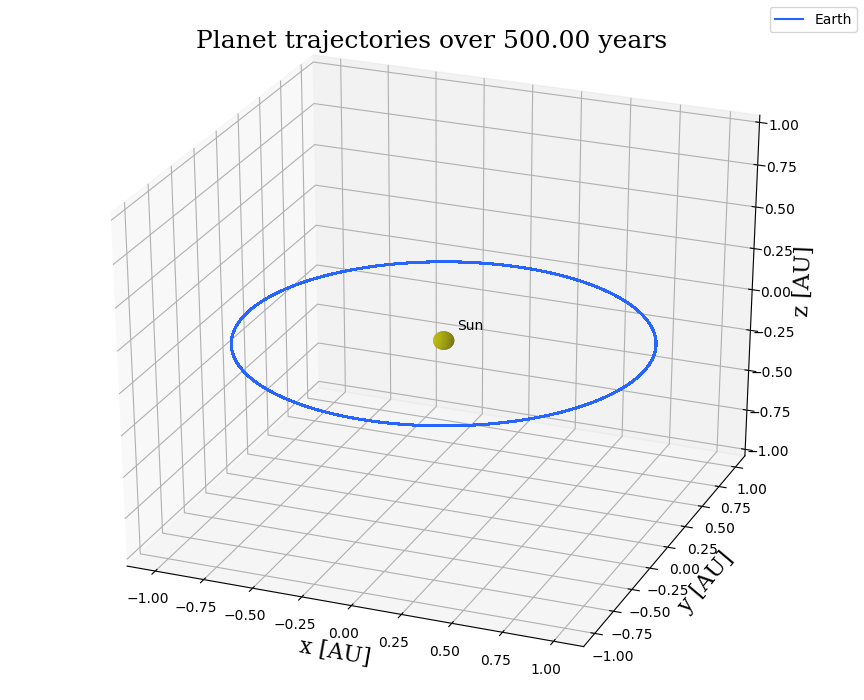
\includegraphics[scale = 0.6]{earth_sun_circular_3D.png}}
 \caption{Figure shows the Earths orbit around the Sun over a time period of 500 years using the Verlet algoritm with a timestep $h=1$ hour.}
 \label{fig:circular plot}
\end{figure}
%Verlet har blitt brukt, ikke sant Jostein?? Ja, det stemmer.
%Har vi brukt initsielle betingelser [1,0,0] og [0, 2pi, 0] i dette plottet?? Yes.



\noindent We want to find the escape velocity, $v_e$, the Earth needs to escape the gravitational forces from the Sun both analytically and numerically in our two body system. To find $v_e$ analytically we utilize equation \eqref{v_e} and plug in the mass of the Sun and the distance between the Earth and the Sun. This gives us that $v_e$ must be equal to or larger than $\pm 8.9112 \frac{AU}{year}$ . \\
%Dette må være feil enhet, hastighet bør vel være AU/year
%Jeg hadde $\frac{AU^3}{kg \hspace{0.1cm} year^2}$ -Trude

\noindent To put this in other words, we have to multiply the velocity of $2\pi$ with a factor 1.41826 to arrive at the lower limit of the escape velocity for the Earth in the Sun-Earth system. Here we have assumed that the distance between the Earth and the Sun is exactly equal to 1.0 A.U. \\
%Nå ble det mer riktig...

%how I calculated it; sqrt(1.9852e-29*2e30*2). This answer is per unit mass.. 


\noindent Numerically we have found that by initializing the Earth with position $\mathbf{r}=$ [1AU, 0, 0] and velocity $\mathbf{v}$ [0, 2*pi, 0], the Earth will escape the Sun's gravitational influence if we multiply the initial velocity in the y-direction by a factor $\sim 1.412$. Here we have taken great effort in extending the simulation interval (sufficient increase in $t_{final}$) to be certain that the Earth does not reenter the Suns gravitational influence through a very large elliptical orbit. We have used $t_{final} = 40 000$ years and a time step $h=10$ days.\\ 

\noindent Our numerical results differs slightly from the analytical result. This is most likely due Taylor expansion truncation error or some loss of numerical precision, i.e. round-off errors. As we remember from table \ref{tab:energy_verlet}, the kinetic energy does not remain completely constant throughout the computation. As $E_k\propto v^2$, we would expect some imprecision in calculations of $v$ after a considerable amount of time steps. The relative error is however of order, $10^{-3}$ which we find quite acceptable considering our rather large time step.\\

\noindent Next we want to investigate what would happen if we change the gravitational force given in equation \eqref{Gforce} to;
\begin{equation}
		\label{altGforce}
        F = \frac{ G M_S M_E}{r^\beta}
\end{equation}
\noindent where we let $\beta$ vary in the interval [2,3]. Figure \ref{fig:beta_gravity} shows the Earth's trajectory for $\beta=2.5$ and for $\beta = 3$. \\

\begin{figure}[ht]
 \centerline{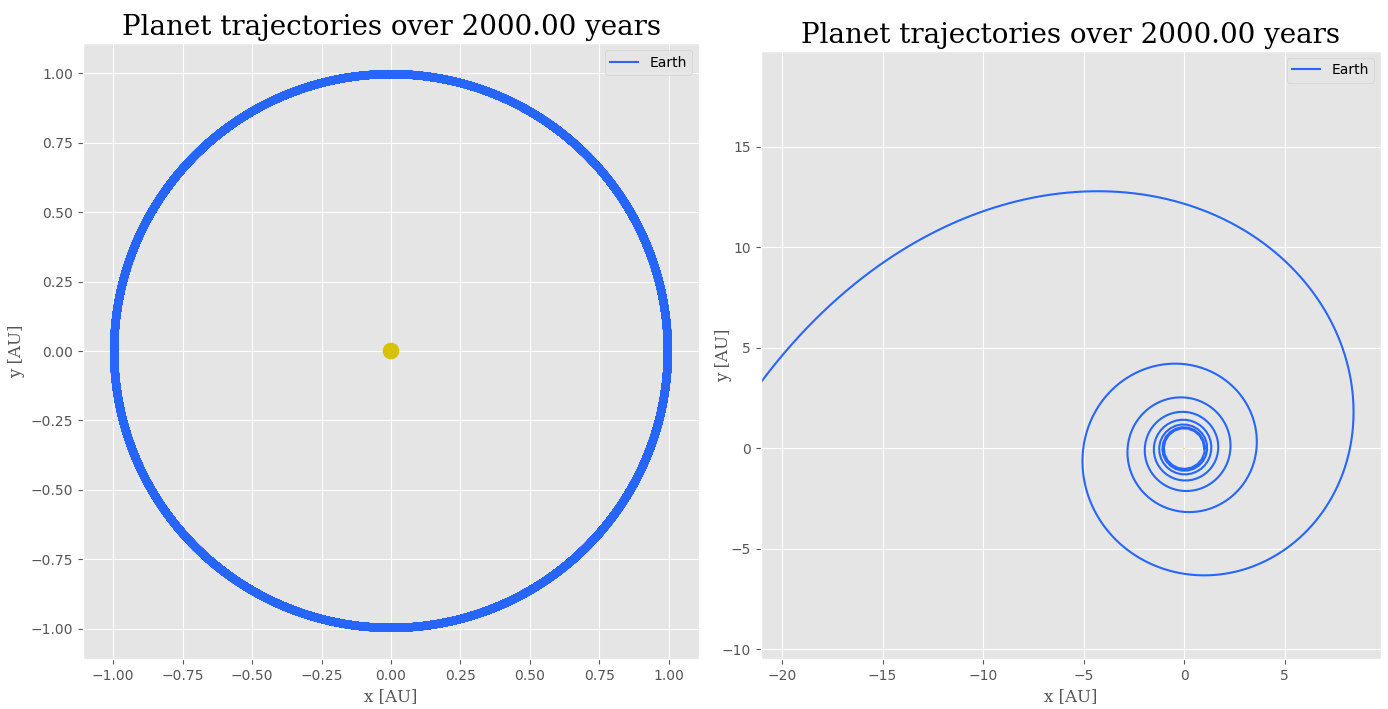
\includegraphics[scale = 0.45]{earth_sun_beta_combined.png}}
 \caption{Time evolution over 2000 years for the sun-earth system using $\beta=2.5$ (left panel) and $\beta=3$ (right panel). The simulation was run with a time step of $5$ days.}
 \label{fig:beta_gravity}
\end{figure}

\noindent For $\beta=2.5$ the Earth starts spiraling slowly outwards, but is still orbiting the Sun after 2000 years. As the gravitational force is proportional to $1/r^\beta$ and the distance between the Sun and the Earth is quite large, the gravitational force will decrease as $\beta$ increases. This accounts for the outwards spiraling of the Earth in the left part of figure \ref{fig:beta_gravity}. Increasing $\beta$ to $3$ makes the Earth start spiraling quickly, and after 2000 years the Earth even seems to have escaped the gravitational pull of the Sun. As we remember from \eqref{v_e}, the escape velocity of the Earth is given by
\begin{equation}
   \label{v_e_beta}
   v_e \geq \sqrt{\frac{2GM}{r^{\beta-1}}}
\end{equation}
Increasing $\beta$ thus leads to a smaller escape velocity, eventually making it possible for the Earth to escape the Sun's gravitational pull for an initial speed of $v=2\pi$ AU/year.


%Maybe include a plot.

%Can here compare whole solarsystem with a=fpipiM/r^4 and  a=fpipiM/r^3 
%--> we will probably observe that planets far awAy slow down their acc and planets orbeting closer the the earth to the sun will increase their acc. 

%Need to rewrite the above section - ODA





%-----------------------------------------------------------------------------------
%-----------------------------------------------------------------------------------
\subsection{The Three Body System}
So far we have seen that when utilizing the Verlet velocity solver, the Earth's motion is relatively stable and constant in time as we can see in figure \ref{fig:circular plot}.

\begin{figure}[ht]
 \centerline{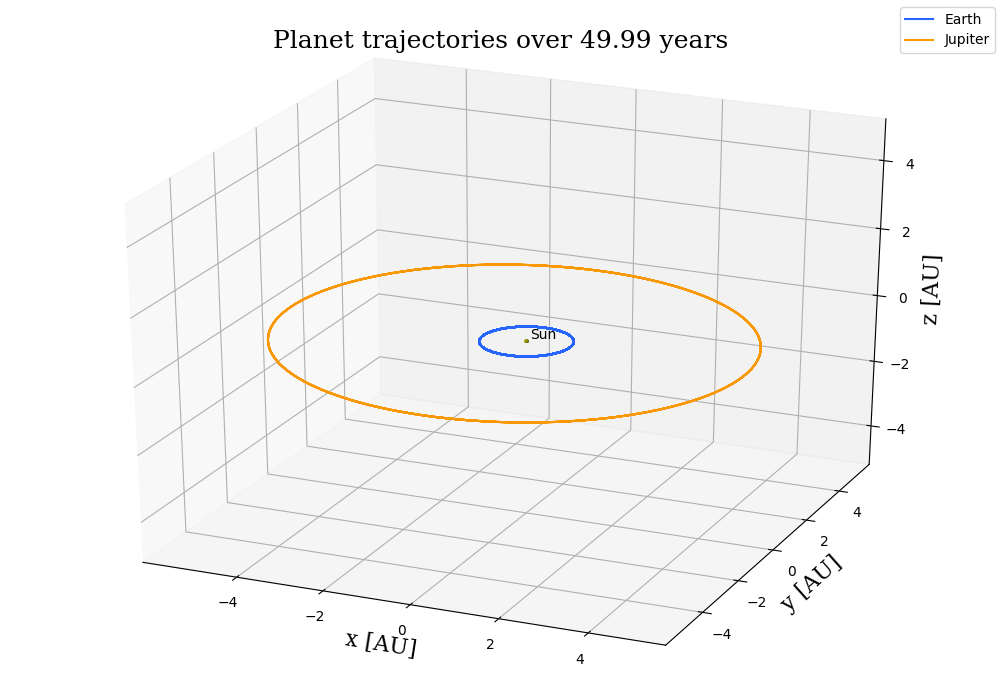
\includegraphics[scale = 0.55]{three_body_fixedsun_nasa_3D.png}}
 \caption{Figure showing the Earth's and Jupiter's orbits around the Sun, which is kept fixed at origin, over a time period of almost 50 years.}
 \label{fig:three body}
\end{figure}

\noindent Now we want to extend our Solar System to include a third body, namely Jupiter. We will continue to keep the Sun fixed in the center of our system and are interested in taking a closer look at how Jupiter, the largest planet in our solar system, influences the motion of the Earth. Plot \ref{fig:three body} shows the orbits of Earth and Jupiter. Here we have used initial conditions for the planets velocity and position collected from Nasa's website: \url{https://ssd.jpl.nasa.gov/horizons.cgi?CGISESSID=173099c92a870c8502c247317aa137a6&s_type=1#top} from October 5. \\

\noindent Figure \ref{fig:three body} shows that the Solar System remains stable when adding Jupiter, which is as we expected. The question now is: what would happen if we increased the mass of Jupiter by a factor of 10 or even a factor of 1000? The results are plotted in figure \ref{fig:jupiter mass}. \\

\begin{figure}[ht]
 \centerline{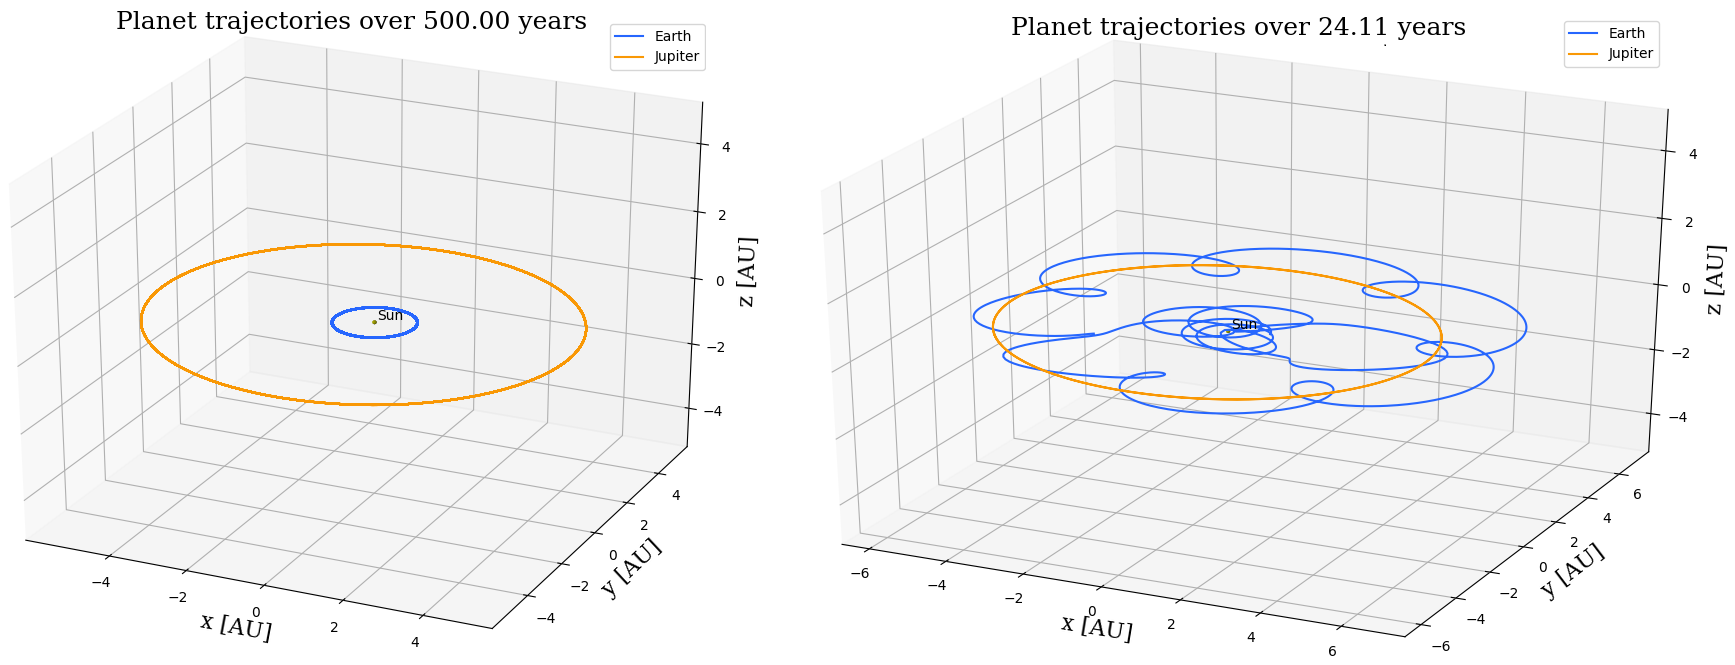
\includegraphics[scale = 0.4]{jupiter_combined_3D.png}}
 \caption{Figure showing the resulting orbits of Earth and Jupiter when we change Jupiter's mass by a factor 10 (left) and 1000 (right). Here we have used a timestep, $h$, equal 3 min. We see clearly from the right plot that changing Jupiter's mass by a factor 1000 has dramatic consequences for the dynamics of our three body system. The reason for 24 years in right panel is for readability and to avoid too much clutter.}
 \label{fig:jupiter mass}
\end{figure}

\noindent We see from figure \ref{fig:jupiter mass} that changing Jupiter's mass by a factor of ten has little influence on the orbits,  but it will of course influence the acceleration of Jupiter as we see from equation \ref{three ax} because the factor $\frac{M_J}{M_S}$ will yield a larger value. This results in a slight increase in Jupiter's orbital velocity thereby decreasing Jupiter's turnaround. This effect will increase proportionally when we increase Jupiter's mass with a factor of one thousand. \\
%Har dere et bedre ord for turnaround??
%Har dere noen tanker om hvilke konsekvender dette har???
%Jeg tenker at dette resulterer i at jupiter går hurtigere i banen sin - mindre omløpstid = turnaround??
%Det kan være at det er en liten forskjell i radiusen til oribiten eller bare beveger den seg raskere??

\noindent From the right plot in figure \ref{fig:jupiter mass} we see that changing Jupiter's mass by a factor 1000 has dramatic effects on the dynamics of our three body system. And this is no surprise, Jupiter's mass is about $1/1000$ of the Sun's mass, so increasing Jupiter's mass by a factor 1000 leaves the mass of Jupiter at about the same size as the mass of the Sun. And as we see the Earth starts alternating between orbiting the Sun and Jupiter, but seemingly mainly becoming a moon of Jupiter. Think about the consequences this would have for life here on Earth. An animation of the dramatic change is uploaded to YouTube at \url{https://youtu.be/sQuR-t25Zhw}. \\

%-----------------------------------------------------------------------------------
%-----------------------------------------------------------------------------------
\subsection{The Solar System}

%For all planets, include link to youtube showing the animation of the whole system-- INCLUDE YOUTUBE link to video of Whole Solar System Simulation  - HVIS VI TRENGER DET??. KANSKJE DET HOLDER MED M_J * 1000 VIDEOEN?? 

\noindent To create a model of the whole Solar System, we have expanded the equation in \eqref{three ax} to include all planets. The Sun will also be treated as a planet in our further calculations. Here we have used initial conditions given by Nasa's website for 5. October 2017. As a start we wish to keep the Sun as the mass center and fixed in origin. Figure \ref{fig:solarsys fixed sun} shows the resulting orbits over a time period of 500 years where we have used a time step, $h$, of one day. Here it is possible to see that the bodies classified as planets (not Pluto though) in our solar system mainly orbit the Sun in the equatorial plane. This indicates that performing our simulation for only two spatial directions, the xy-plane, will result in a fairly good representation of our solar system and this will of course save the number of FLOPs needed, thereby reducing CPU time.  \\


\begin{figure}[ht]
 \centerline{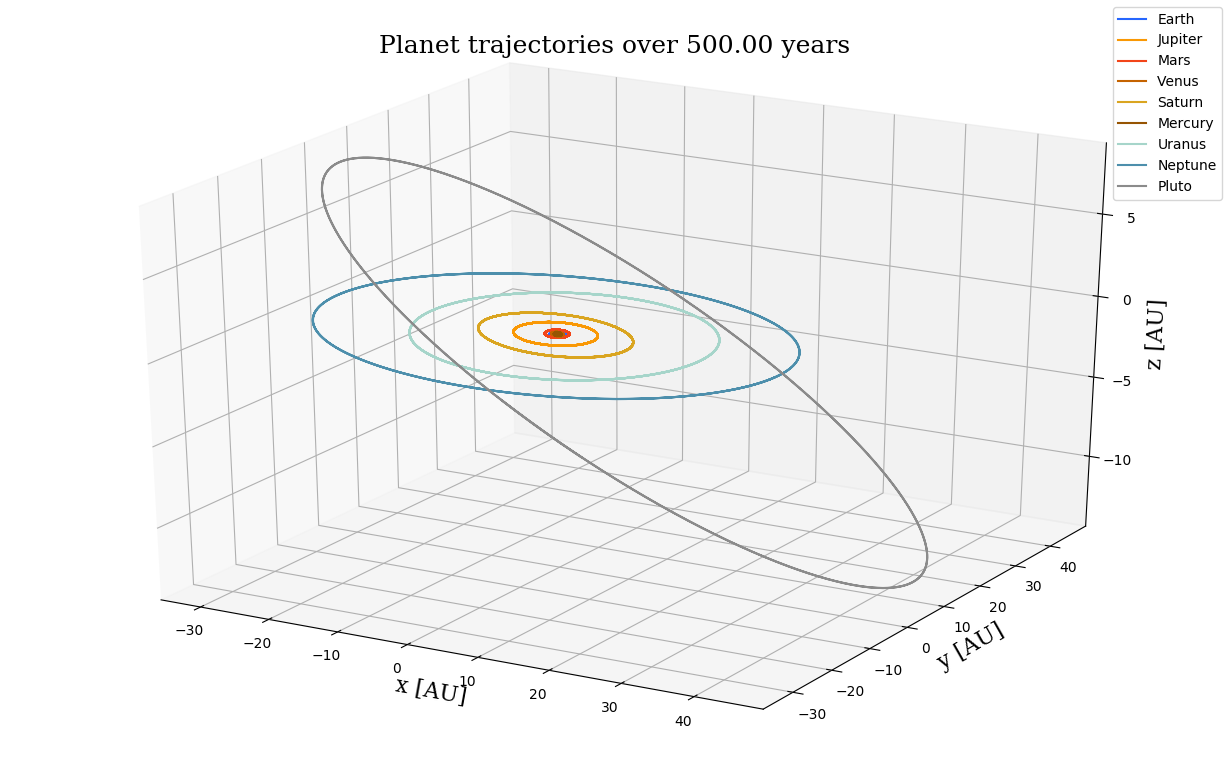
\includegraphics[scale = 0.55]{solar_system_fixedsun_nasa_3D.png}}
 \caption{Figure shows the evolution of our solar system, included Pluto, when we use the Sun fixed in origin throughout our simulation (moving sun gives almost exact same figure).}
 \label{fig:solarsys fixed sun}
\end{figure}

\noindent To make the calculations as realistic as possible within the limits of our approximation, we want to give the Sun an initial velocity so that the total momentum of our system is exactly equal to zero as given by \eqref{eq:sun_init_v}. Doing this will prevent the solar system from getting a net velocity in some direction. We start our calculations with the Sun in the origin, but now with the initial velocities that reduces the total momentum of the system to zero. Figure \ref{fig:sun_osci} shows the resulting motion of the Sun when it is given an initial velocity and is influenced by gravitational forces. We see that the Sun is orbiting in close proximity to the origin and well within (roughly one fifth of) the radius of the Sun (about 0.05 AU). Studying the motion of the Sun, it would thus not seem to have circular orbits, but rather to 'wobble' around about its center of mass. \\

\begin{figure}[ht]
 \centerline{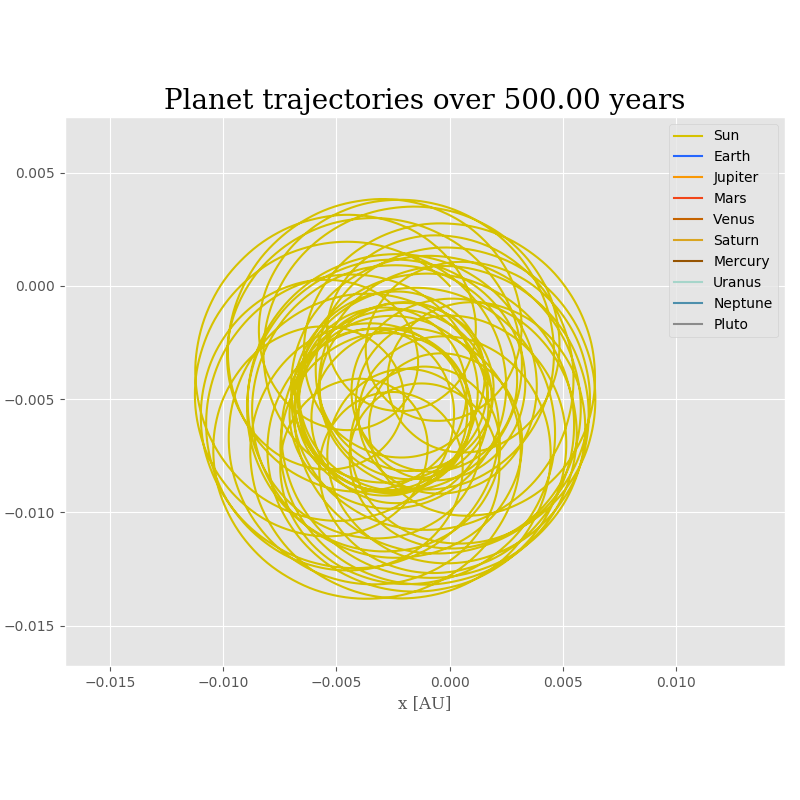
\includegraphics[scale = 0.6]{sun_oscillations.png}}
 \caption{ Figure shows the resulting motion of the Sun when we give the Sun an initial velocity that makes the total  momentum of the system equal to zero. Here we have used a timestep, $h$, equal to 0.1 days and zoomed in on the central areas of our solar system to better visualize the Suns motion.}
 \label{fig:sun_osci}
\end{figure}

\noindent Our observation that the Sun only orbits well within its real radius, indicates that putting the Sun at rest in origin is a good approximation when we are only interested in the dynamics of the orbiting bodies in our solar system. Especially since we have already made the quite crude simplification where we treat all the bodies as point particles. A further argument is that when we find the mass centers position, the returning coordinates are quite close to the origin and within the radius of the Sun, with $r_{MC} \sim [ -0.0023, -0.0055, 0.00013]$. We also know that the Sun contains 99.86\% of our solars systems total mass \cite{sun}. So keeping the Sun fixed in origin looks like an attractive option as this lets us see the planets orbits (here also Pluto is included) clearly and saves us FLOPs and CPU time. \\

\noindent An animation of the full solar system (sun not fixed) simulation over 250 years can be found at \url{https://youtu.be/Gi8v0cHA5IM}. We also wanted to explore the case of a massive celestial body (perhaps a large asteroid of some sort) with mass of 1/20 of that of the sun entering our solar system with some velocity. We observed that the solar system responded quite dramatically and the gravitational pull towards the asteroid disturbed the entire solar system. This gives an indication of what might happen if such an event were to occur. An animation can be seen at \url{https://youtu.be/PtQ8x0xHPpQ}.

%initbet. for hastighet til solen: 0.001842214  -0.0020190128  -4.2437519e-05
%Og her er koordinatene til massensenteret: -0.002253506 -0.0055375304 0.00012903377

%--------------------------------------------------------------------------------------
%--------------------------------------------------------------------------------------
\subsection{The Perihelion of Mercury}
So far, our simulations has not included any corrections from general relativity.

\begin{table}[ht]
\begin{center}
  \begin{tabular}{| l | l | l | l |}
  \hline
     With general relativity & Newtonian \\[0.05cm]\hline
       & \\
     43.025 & 0.6032 \\
     \hline
  \end{tabular}
\end{center}
\caption{The perihelion angle (in arc seconds) of Mercury after 100 years with and without general relativity correction to the law of gravitation. We have used a time step $h=8.64$ seconds}
\label{tab:perhileon}
\end{table}

We now want to compute the perihelion angle of Mercury with and without the general relativity correction to the law of gravity \eqref{GR}. The result is presented in table \ref{tab:perhileon} , where we used a time step of 8.64 seconds. As can be seen in the table, the computed perihelion angle when general relativity corrections are taken into account, is quite close to the observed angle of 43''. The perihelion angle when using only Newton's law of gravitation, is about two orders of magnitude smaller than the observed one. It seems that the perihelion angle of Mercury cannot be explained using only Newton's law of gravitation, but by also including general relativity.

%====================================================================================
%====================================================================================
\section{Concluding remarks}
\noindent Science has made many groundbreaking discoveries through the ages. Among these, the discovery of the Sun as the center of the Solar System is perhaps the most famous. One can only imagine how difficult and extremely time consuming it must have been to find an approximate model of the motion of the planets back then. Fortunately, technology has moved a lot forwards since then, and it is now possible to find approximate solutions to differential equations in a matter of minutes or even seconds (depending of course on the chosen number of time steps) by solving the equations numerically.\\

\noindent In this project our goal was to build a model of the Solar system using numerical methods, namely Euler and Velocity Verlet. Using known physical properties of the Solar System allowed us to compare the exactness of the methods. In section \ref{sec:testing} we saw that the Verlet method is superior to the Euler when it comes to conservation of energy, and that it also to a high degree conserves angular momentum. Table \eqref{tab:timing} also shows that the difference of time used by both methods is quite small, leading us to conclude that Velocity Verlet is by far the superior method. In addition, as discussed in section \ref{sec:methods}, the Verlet algorithm is a higher order numerical scheme. \\

\noindent Throughout the project we have also experimented with changing different parameters, most notably the mass of Jupiter and the dependency of the radius in the gravitational force. Figure \ref{fig:beta_gravity} and figure \eqref{fig:jupiter mass} show how dramatic the consequences of this would be. Most of us take the stability of stability of the Solar System as granted (overlooking of course the eventual 'death' of the Sun). Our results in this project show how amazing it is that the planets orbit the Sun in such an ordered manner, as small changes to velocities, mass or the gravitational law, severely alters the motion.\\

\noindent Were one to work further on this project, it would be interesting to take the diminishing mass of the Sun into consideration, and study what effect this would have on the motion of the planets after millions of years. Including the moons of the different planets would also be interesting, as this would lead to an even more realistic model. With more time we would also have liked to perform more timing tests for varying number of bodies $N$ to confirm the $N^2$ cost dependency on the number of bodies, but also to observe that the difference between Euler and Verlet time usage would shrink with increasing $N$. And although we were pleased by the precision of the Velocity Verlet algorithm (especially considering the time efficiency of the method) it might be worthwhile to look into a numerical method of a higher order error term, e.g. Runge Kutta 4, to check if this would lead to a considerably improvement of the precision.

\pagebreak

\bibliography{sample}{}
\bibliographystyle{plain}

\end{document}